\documentclass[conference]{IEEEtran}
\IEEEoverridecommandlockouts
% The preceding line is only needed to identify funding in the first footnote. If that is unneeded, please comment it out.
\usepackage{cite}
\usepackage{amsmath,amssymb,amsfonts}
\usepackage{algorithmic}
\usepackage{graphicx}
\usepackage{textcomp}
\usepackage{xcolor}
\usepackage{tabularx}
\def\BibTeX{{\rm B\kern-.05em{\sc i\kern-.025em b}\kern-.08em
    T\kern-.1667em\lower.7ex\hbox{E}\kern-.125emX}}
\begin{document}

\title{A Survey on Multi-modal Emotion Detection Techniques\\

}


\author{
\IEEEauthorblockN{1\textsuperscript{st} Prof. Chintan R. Chatterjee}
\IEEEauthorblockA{\textit{dept. name of organization (of Aff.)} \\
\textit{name of organization (of Aff.)}\\
City, India \\
email address or ORCID}
\and
\IEEEauthorblockN{2\textsuperscript{nd} Nihir Shah}
\IEEEauthorblockA{\textit{dept. name of organization (of Aff.)} \\
\textit{name of organization (of Aff.)}\\
City, India \\
email address or ORCID}
\and
\IEEEauthorblockN{3\textsuperscript{rd} Dr. Brijesh S. Bhatt}
\IEEEauthorblockA{\textit{dept. name of organization (of Aff.)} \\
\textit{name of organization (of Aff.)}\\
City, India \\
email address or ORCID}

\and


\IEEEauthorblockN{4\textsuperscript{th} Sahil Bhatt}
\hspace{9cm} 
\IEEEauthorblockA{\textit{dept. name of organization (of Aff.)} \\
\textit{name of organization (of Aff.)}\\
City, India \\
email address or ORCID}

\and
\IEEEauthorblockN{5\textsuperscript{th} Smit Chandi}
\IEEEauthorblockA{\textit{dept. name of organization (of Aff.)} \\
\textit{name of organization (of Aff.)}\\
City, India \\
email address or ORCID}
}
\maketitle
\begin{abstract}
Emotion detection and recognition have significant implications for human-computer interaction and multimedia analysis. The unimodal approach have been a primary source of features that are required for the detection until recent years where we have seen trends of multi-modal approach to affective computing. In this paper, we present those techniques and how the multi-modal systems are changing the...
\end{abstract}
\begin{IEEEkeywords}
component, formatting, style, styling, insert
\end{IEEEkeywords}

\section{Introduction}
The analysis of emotions in artificial intelligence is crucial for creating empathetic systems. The utilization of unimodal or single modality-based strategies have played a crucial part in the genesis of emotion detection systems. Drawing from the examination of individual sources of data like facial expressions\cite{r1}\cite{r2}, vocal inflections\cite{r4}\cite{r5}or textual inferences\cite{r3}, these methodologies have furnished fundamental understandings into the domain of emotion recognition. Nevertheless, as our comprehension of the intricacy of human emotions has grown, the constraints associated with depending solely on a singular type of information have become progressively apparent.

The complex and intricate web of human emotions, with their diverse and nuanced characteristics, cannot be adequately encompassed within the confines of a singular perspective, brain responses constitute emotion or the body expression of emotion and that emotion feeling is a consequence of the neurobiological (body) expression\cite{r6}. Emotions are not isolated entities; they are formed through a multitude of interconnected elements, each embodying a unique form of communication. While facial expressions hold immense value, they alone may not unveil the entirety of one's emotional landscape. Similarly, vocal cues provide valuable clues, yet they may lack the profoundness required for a thorough examination\cite{r7}. 

The acknowledgment of emotions' intricate nature has sparked the emergence of multi-modal techniques in analyzing emotions. By incorporating information from different sources, including facial expressions, voice, and text, a comprehensive and intricate portrayal of emotional states is created. This harmonious fusion of diverse cues allows for a more precise and refined understanding of emotions, surpassing the constraints of individual modalities.Multi-modal approaches combine data from various sources, such as facial expressions, voice, and text, resulting in improved accuracy and better addressing the complexity of emotions. Emotions are intricate psychological phenomena that deeply impact human interactions. Being able to recognize and understand them enhances meaningful communication. While single-mode recognition may struggle, combining cues from multiple senses effectively captures emotional states. Therefore, current efforts are focused on developing multi-modal systems that can accurately identify human emotions, ushering in a new era of responsive AI interactions.

Multimodal emotion detection in machine learning refers to the task of recognizing and understanding human emotions by using multiple sources of data or modalities. \cite{hina2022multimodal}
The modalities can  be provided in various ways such analysing the text, audios, videos, images, Physiological Signals and many more.

Machine learning techniques used in multimodal emotion detection include fusion methods, where information from different modalities is combined into a unified representation, and multi modal deep learning models, which integrate various types of neural networks to process different modalities simultaneously \cite{joshi2022cogmen}. For integrating information from various sources, multimodal deep learning architectures that can handle inputs from several modalities are used. These could include parallel CNNs, RNNs, or transformers for several modalities, followed by multimodal fusion layers \cite{sharafi2022novel}. 

\begin{figure}[htbp]
\centerline{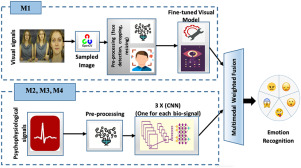
\includegraphics{Multimodal.png}}
\caption{Multimodal Classification for Emotion Detection.\cite{KUMAR2022104483}}
\label{fig}
\end{figure}

The initial stage in multimodal emotion identification is to efficiently fuse information from diverse modalities. Merge the raw data from all modes into a single input representation. Combining text embeddings, audio features, and image features. Textual data can be processed using Recurrent Neural Networks (RNNs), Long Short-Term Memory (LSTM) networks, or Transformers. Convolutional Neural Networks (CNNs) or Recurrent Neural Networks (RNNs) are neural networks that are used to process audio signals or spectrogram images. Convolutional Neural Networks (CNNs) like ResNet or VGG are used to process pictures or video frames \cite{huang2019multimodal}.

\section{Types of Data in Emotion Detection}

Facial emotion detection using images is a technology that involves analyzing facial expressions in images or videos to determine the emotions being displayed by individuals. The first step is to identify and locate the faces within the image. This is often done using techniques like Haar cascades, deep learning-based methods (e.g., Convolutional Neural Networks or CNNs), or other advanced computer vision algorithms.  Once faces are detected, relevant features are extracted from the face regions. After extracting features, machine learning techniques are employed to classify the detected emotions. Various algorithms can be used for this, such as Support Vector Machines (SVMs), Random Forests, or more commonly, deep learning models like CNNs.

Emotion detection using voice, also known as speech emotion recognition, is another fascinating application of machine learning. Choose a suitable machine learning model for emotion detection. Recurrent Neural Networks (RNNs), Convolutional Neural Networks (CNNs), and more advanced models like Long Short-Term Memory (LSTM) networks or Gated Recurrent Units (GRUs) are commonly used for sequential data like audio.

Emotion detection using video data involves analyzing facial expressions and other visual cues to infer the emotional state of individuals. Detect and track faces within each video frame. This can be achieved using techniques like Haar cascades, deep learning-based object detection models (e.g., Faster R-CNN, SSD), or facial landmark detection models.

\begin{figure}[htbp]
\centerline{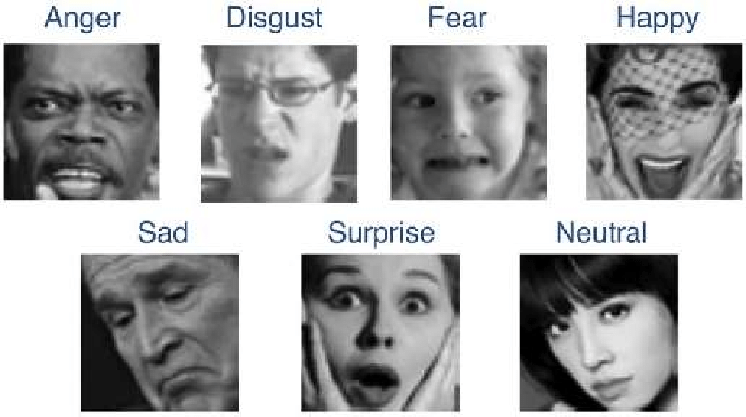
\includegraphics[scale=0.35]{Facial_Emotion.png}}
\caption{Facial Emotion.}
\label{fig}
\end{figure}

Emotion detection using voice, also known as speech emotion recognition, involves analyzing audio signals (such as spoken words or speech segments) to determine the emotional state of the speaker.  The first step is to extract relevant features from the audio signal. These features can include acoustic characteristics such as pitch, intensity, rhythm, spectral content, and more. These features capture the patterns and nuances in the voice that are associated with different emotions. After extracting features, machine learning techniques are used to classify the detected emotions. Similar to facial emotion detection, algorithms like Support Vector Machines (SVMs), Random Forests, and deep learning models are commonly employed for this task \cite{s19122730}.

MFCCs are commonly used features for speech processing tasks. They capture the spectral characteristics of the voice signal and have been successful in representing emotional information.

Emotion detection from voice can be challenging due to factors like variations in accents, speech rate, background noise, and individual differences in speech patterns. Robustness to these factors requires careful data preprocessing, feature engineering, and model design. To improve the model's performance over time, you can collect user feedback and retrain the model with additional data. This can help the model adapt to different user preferences and variations.

\section{Multi-modal Parametrization}
\subsection{Speech}
Speech feature extraction is the process of converting a speech signal into a set of features that can be used by a machine learning model to perform tasks such as speech recognition, speaker identification, language modeling  and emotion detection.  Some of the common techniques employed for emotion detection are:

\textbf{Mel-frequency cepstral coefficients (MFCCs)}: MFCCs\cite{r17} are a set of features that are designed to mimic human auditory perception. They are calculated by filtering the speech signal into a number of frequency bands, and then extracting the cepstral coefficients from each band. MFCCs are one of the most widely used speech feature extraction methods, and have been shown to be very effective for speech recognition tasks.

\textbf{Linear predictive coefficients (LPCs)}: LPCs\cite{r18} are a set of features that are calculated by modeling the speech signal as a linear filter. LPCs are often used in conjunction with MFCCs to improve the performance of speech recognition systems.

\textbf{Perceptual linear prediction (PLP)}: PLP\cite{r19} is a speech feature extraction method that is similar to LPCs, but it takes into account the non-linear nature of human auditory perception. PLP features have been shown to be effective for speech recognition tasks in noisy environments.


\textbf{Wavelet transform (WT)}: WT\cite{r20} is a mathematical transformation that can be used to decompose a signal into its constituent frequency components. WT features can be used to extract information about the temporal and spectral characteristics of a speech signal.



\subsection{Text}
Feature extraction techniques are foundational in the realm of text analysis\cite{r8}, enabling the transformation of unstructured text data into a structured format conducive to computational analysis. These techniques are diverse, each serving a distinct purpose in processing and understanding textual information.
Tokenization\cite{r10} stands as the initial step, segmenting text into individual words or tokens. This forms the fundamental unit for subsequent analysis, enabling the isolation and examination of each component of the text.
TF-IDF\cite{r9} is short form for term frequency-inverse document frequency. TF-IDF is
one of the largely used methods in information retrieval and text mining. TF-IDF is
a weight metric which determines the importance of word for that document. The tf–idf is the product of two statistics, term frequency and inverse document frequency. There are various ways for determining the exact values of both statistics.
Term Frequency (TF) measures the number of times a specific term, denoted as $t$, occurs in a document, denoted as $d$. The frequency increases when a term appears multiple times in the document. TF is calculated as the ratio of the frequency of term $t$ in document $d$ to the total number of terms in that particular document, expressed as:

\[
TF(t,d) = \frac{\text{Number of times term } t \text{ appears in document } d}{\text{Total number of terms in document } d} \tag{1}
\]
While TF measures the frequency of a term, it may not capture the importance of certain terms. Some terms, such as stop words, occur frequently but may not provide significant information. Inverse Document Frequency (IDF) is used to assess the importance of a term. IDF assigns higher importance to terms that occur rarely across documents. IDF is calculated as:

\[
IDF(t) = \log_e \left( \frac{\text{Total number of documents}}{\text{Total number of documents with term } t \text{ in them}} \right) \tag{2}
\]
The final weight of a term $t$ in a document $d$ is computed using the TF-IDF formula:

\[
TF\text{-}IDF(t,d) = TF(t,d) \times IDF(t) \tag{3}
\]

This weighting assigns a value that reflects the importance of a term $t$ within a specific document $d$. Higher TF-IDF scores indicate that a term is both frequent within the document and rare across the entire corpus of documents. This measure is valuable in tasks like text classification and information retrieval.

Another technique widely used is doc2vec.
 The doc2vec model, introduced by Le and Miklov in 2014\cite{r12}, is an extension of the word2vec model\cite{r11} that aims to enhance the learning of embeddings from word sequences. Unlike word2vec, which focuses solely on individual words, doc2vec is capable of representing word n-grams, sentences, paragraphs, or entire documents.
 In comparison to word2vec, which implements the continuous bag of words (CBOW)\cite{r13} and skip-gram (SG) algorithms, doc2vec employs the distributed memory (DM) and distributed bag of words (DBOW) algorithms\cite{r14}. These algorithms enable doc2vec to capture the contextual information and relationship between words within a document, leading to more accurate and meaningful document representations. Doc2vec is a powerful approach that transforms documents into fixed-length, low-dimensional vectors. It consists of a three-layer neural network, comprising an input layer, a hidden layer, and an output layer. This architecture enables doc2vec to capture the semantic meaning of documents and encode them into compact representations. In summary, doc2vec is an advanced model that extends the capabilities of word2vec by considering word sequences and their contexts. By transforming documents into fixed-length vectors, doc2vec provides a powerful tool for various natural language processing tasks, such as text classification, sentiment analysis, and information retrieval. There are two variations of doc2vec: distributed bag of words (DBOW)\cite{r15} and distributed memory (DM)\cite{r16}. The DBOW approach treats each document as a single entity and predicts words randomly sampled from the document. On the other hand, the DM approach takes both the document and its context into account, predicting words based on the combination of the document and its surrounding words.



\section{Techniques Used}

\subsection{Deep Learning techniques used for Emotion Detection}

Transformers are one of the techniques used in the Deep learning framework. The textual data can be processed by the transformers for recognizing the emotions \cite{karatay2022multi},\cite{le2023multi}. 
Transformers are used in sequence transduction. This means that if we want to transform any input sequence to the output sequence, we can use transformers. The applications of transformers include Speech recognizing, text recognition and many more. When the speech is converted into sequence of words, it is given as an input to the transformer. The architecture detects the speech by extracting its features and output of sequence is produced from the transformers. The model attends to all the other words in the sentence and calculates a weighted sum of their representations to create the output representation for each word. it first encode the input sequence into vector representation. This step is called as Encoding \cite{huang2020multimodal}.
To process the input and output sequences, the decoder employs self-attention and cross-attention techniques. Transformers are typically trained using supervised learning with large labeled data sets. After each layer, layer normalization and residual connections are applied. Layer normalization aids in training process stability, while residual connections allow gradients to flow more effectively through the network, eliminating disappearing gradients and making deep models easier to train.\cite{lian2021ctnet} 

\begin{figure}
\centerline{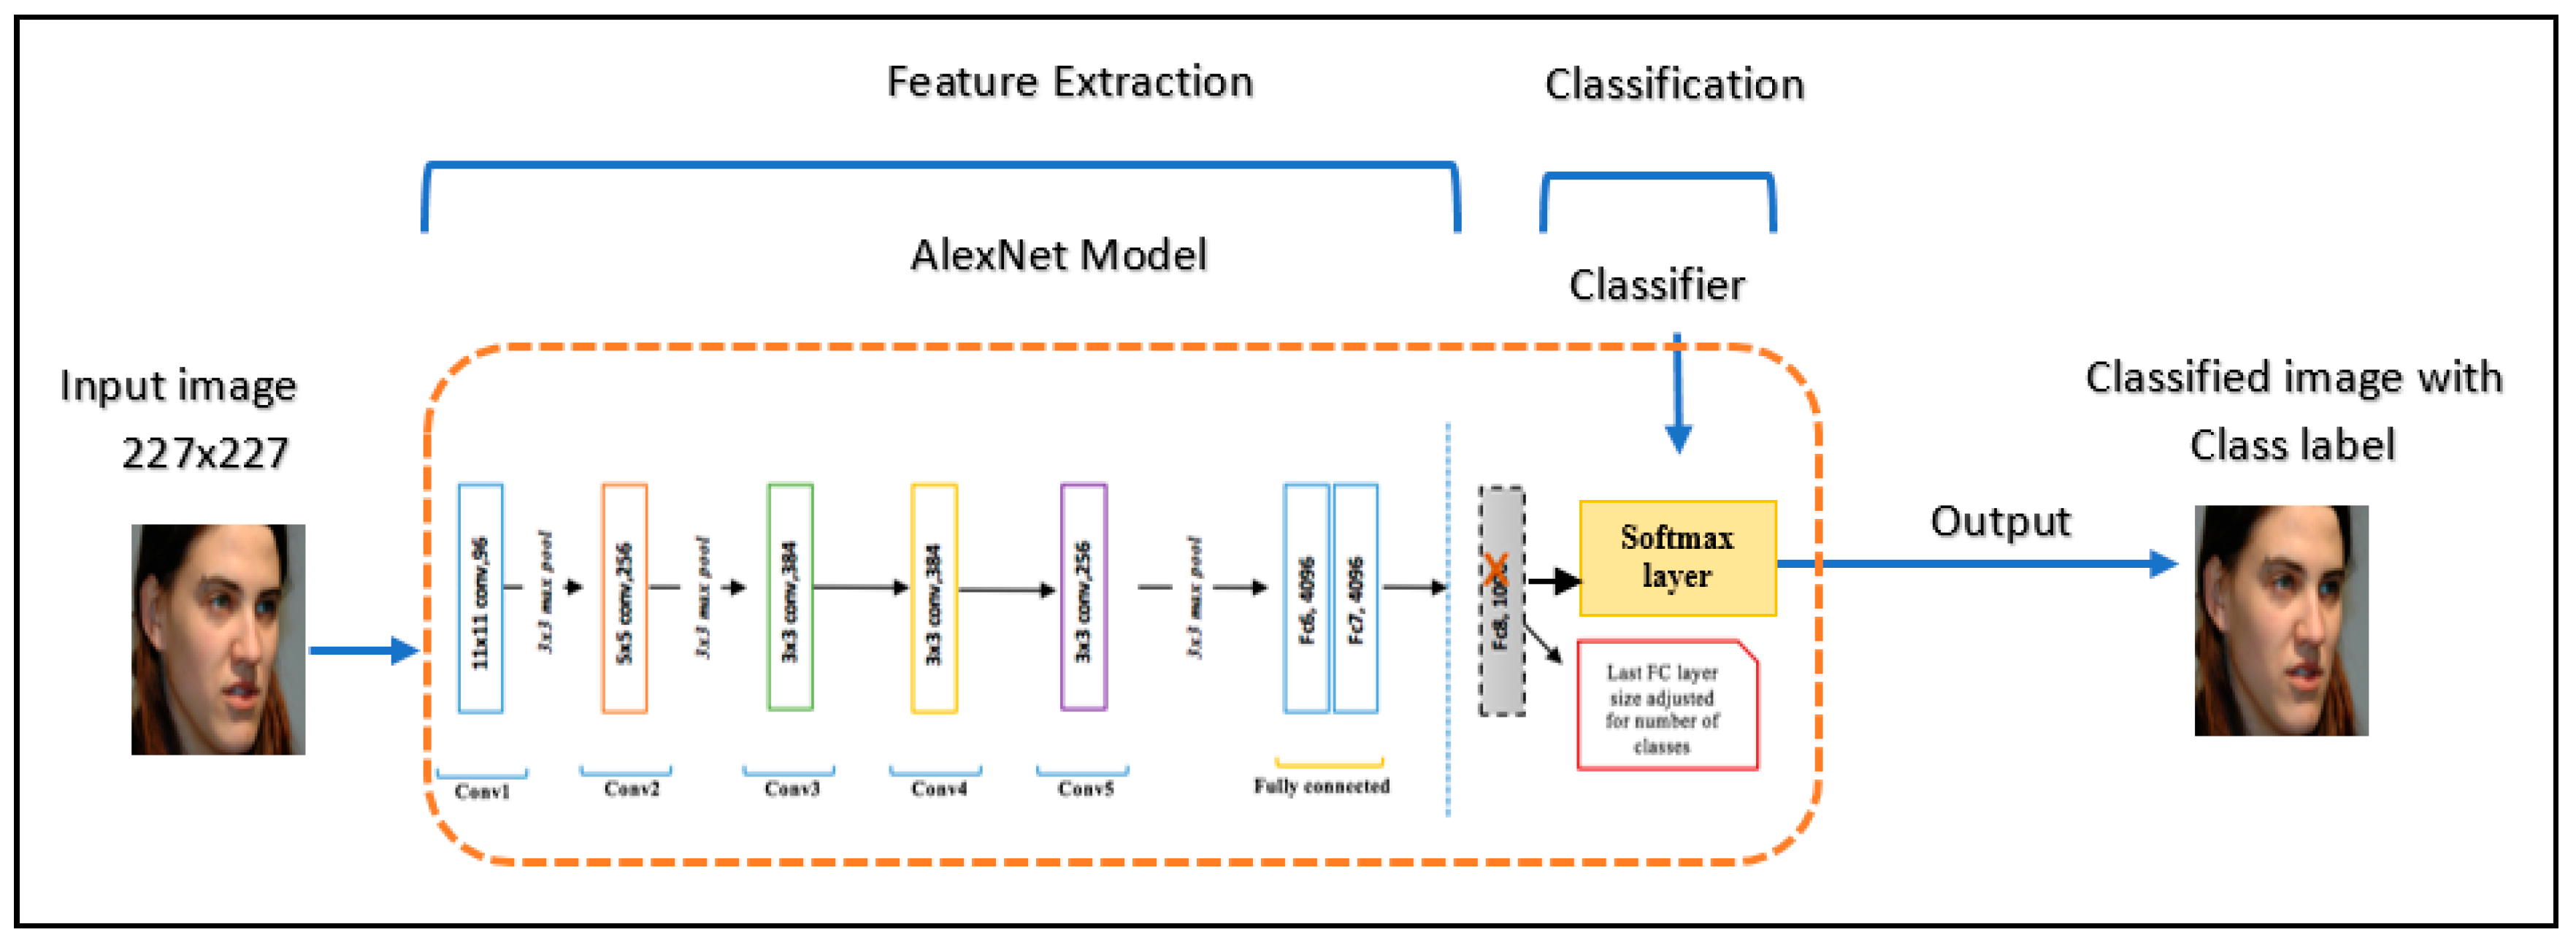
\includegraphics[scale=0.07]{DNNmodel.png}}
\caption{DNN Model \cite{app9204397}}
\end{figure}


GANs can be used for generating realistic data samples in one modality based on the information from other modalities \cite{vidal2023multimodal}, \cite{luo2019gan}. 
Another technique is the Transfer learning. It is the concept in which once the machine learning model has been trained to get the patterns out of the data, the concept of transfer process is used. n the context of emotion detection, transfer learning can be employed to leverage pre-trained models that have been trained on large datasets for tasks like sentiment analysis, language understanding, or image recognition. This approach helps improve the performance of emotion detection models, especially when limited labeled data is available for the specific emotion detection task. This utilizes the information from the trained model to improve its accuracy and is able to perform the task which is relevant to the previous one without training the model. Basically, it is the pre-trained model that can be reused for solving another problem. The BERT model of transfer learning can be used for the text recognition \cite{padi2022multimodal}. 
The Ensemble learning approach of Combining multiple deep learning models, each specialized in a specific modality, can lead to improved performance \cite{salama20213d}. 
Fusion CNNs models can be used to  to combine information from multiple modalities at various levels \cite{zhang2021multimodal}.  Ensemble models combine predictions from multiple individual models to improve overall performance. You can create an ensemble of GRU-based models with different hyperparameters, input representations, or initializations to improve the diversity of predictions and enhance emotion detection accuracy.
Multimodal Attention Mechanisms allow the model to focus on the most relevant parts of each modality when making predictions. Selective fusion of data from several modalities is possible with multimodal attention \cite{zhang2023multimodal}.While not GRUs, TCNs are an alternative architecture for sequence modeling that can be used for emotion detection. TCNs use dilated convolutions to capture long-range dependencies in sequences, making them suitable for tasks where context over longer distances is crucial.
TCNs often use residual connections to mitigate the vanishing gradient problem and improve training stability. Residual connections enable the network to directly learn the residual (difference) between the input and the output of a layer. This facilitates the training of deeper networks. After applying convolutional layers, TCNs often use temporal pooling layers (e.g., max pooling) to downsample the sequence. This helps in reducing the computational complexity and capturing higher-level features. Following the convolutional and pooling layers, TCNs typically have one or more fully connected layers that perform the final classification for emotion detection. These layers aggregate the features learned by the convolutional layers and make predictions based on the context captured in the sequence \cite{zheng2023two}. The final output layer of a TCN is usually a softmax layer that assigns a probability distribution over the emotion classes. This allows the network to make emotion predictions based on the learned features. Ns are trained using backpropagation and gradient descent, just like other neural network architectures. The loss function used for training depends on the task, but for emotion detection, it could be categorical cross-entropy \cite{hu2023multiscale}. During training, the network learns to adjust its parameters to minimize the difference between predicted and actual emotion labels. The advantages of TCNs for emotion detection include their ability to capture long-range dependencies in sequences, their parallel processing of different features, and their potential to handle variable-length sequences. However, like any neural network architecture, the effectiveness of TCNs depends on factors such as the quality and size of the training data, the architecture's hyperparameters, and the task's inherent complexity.

 NLP techniques, such as word embeddings (Word2Vec, GloVe) and recurrent neural networks (RNNs), are used to capture semantic relationships and context in text, aiding emotion detection.
 Electroencephalogram (EEG) signals are analyzed to identify patterns that correspond to emotional states. Machine learning models classify these patterns to detect emotions. Mel-Frequency Cepstral Coefficients (MFCCs) are a common feature extraction technique for speech signals that captures relevant spectral characteristics for emotion recognition.

\begin{figure}[htbp]
\centerline{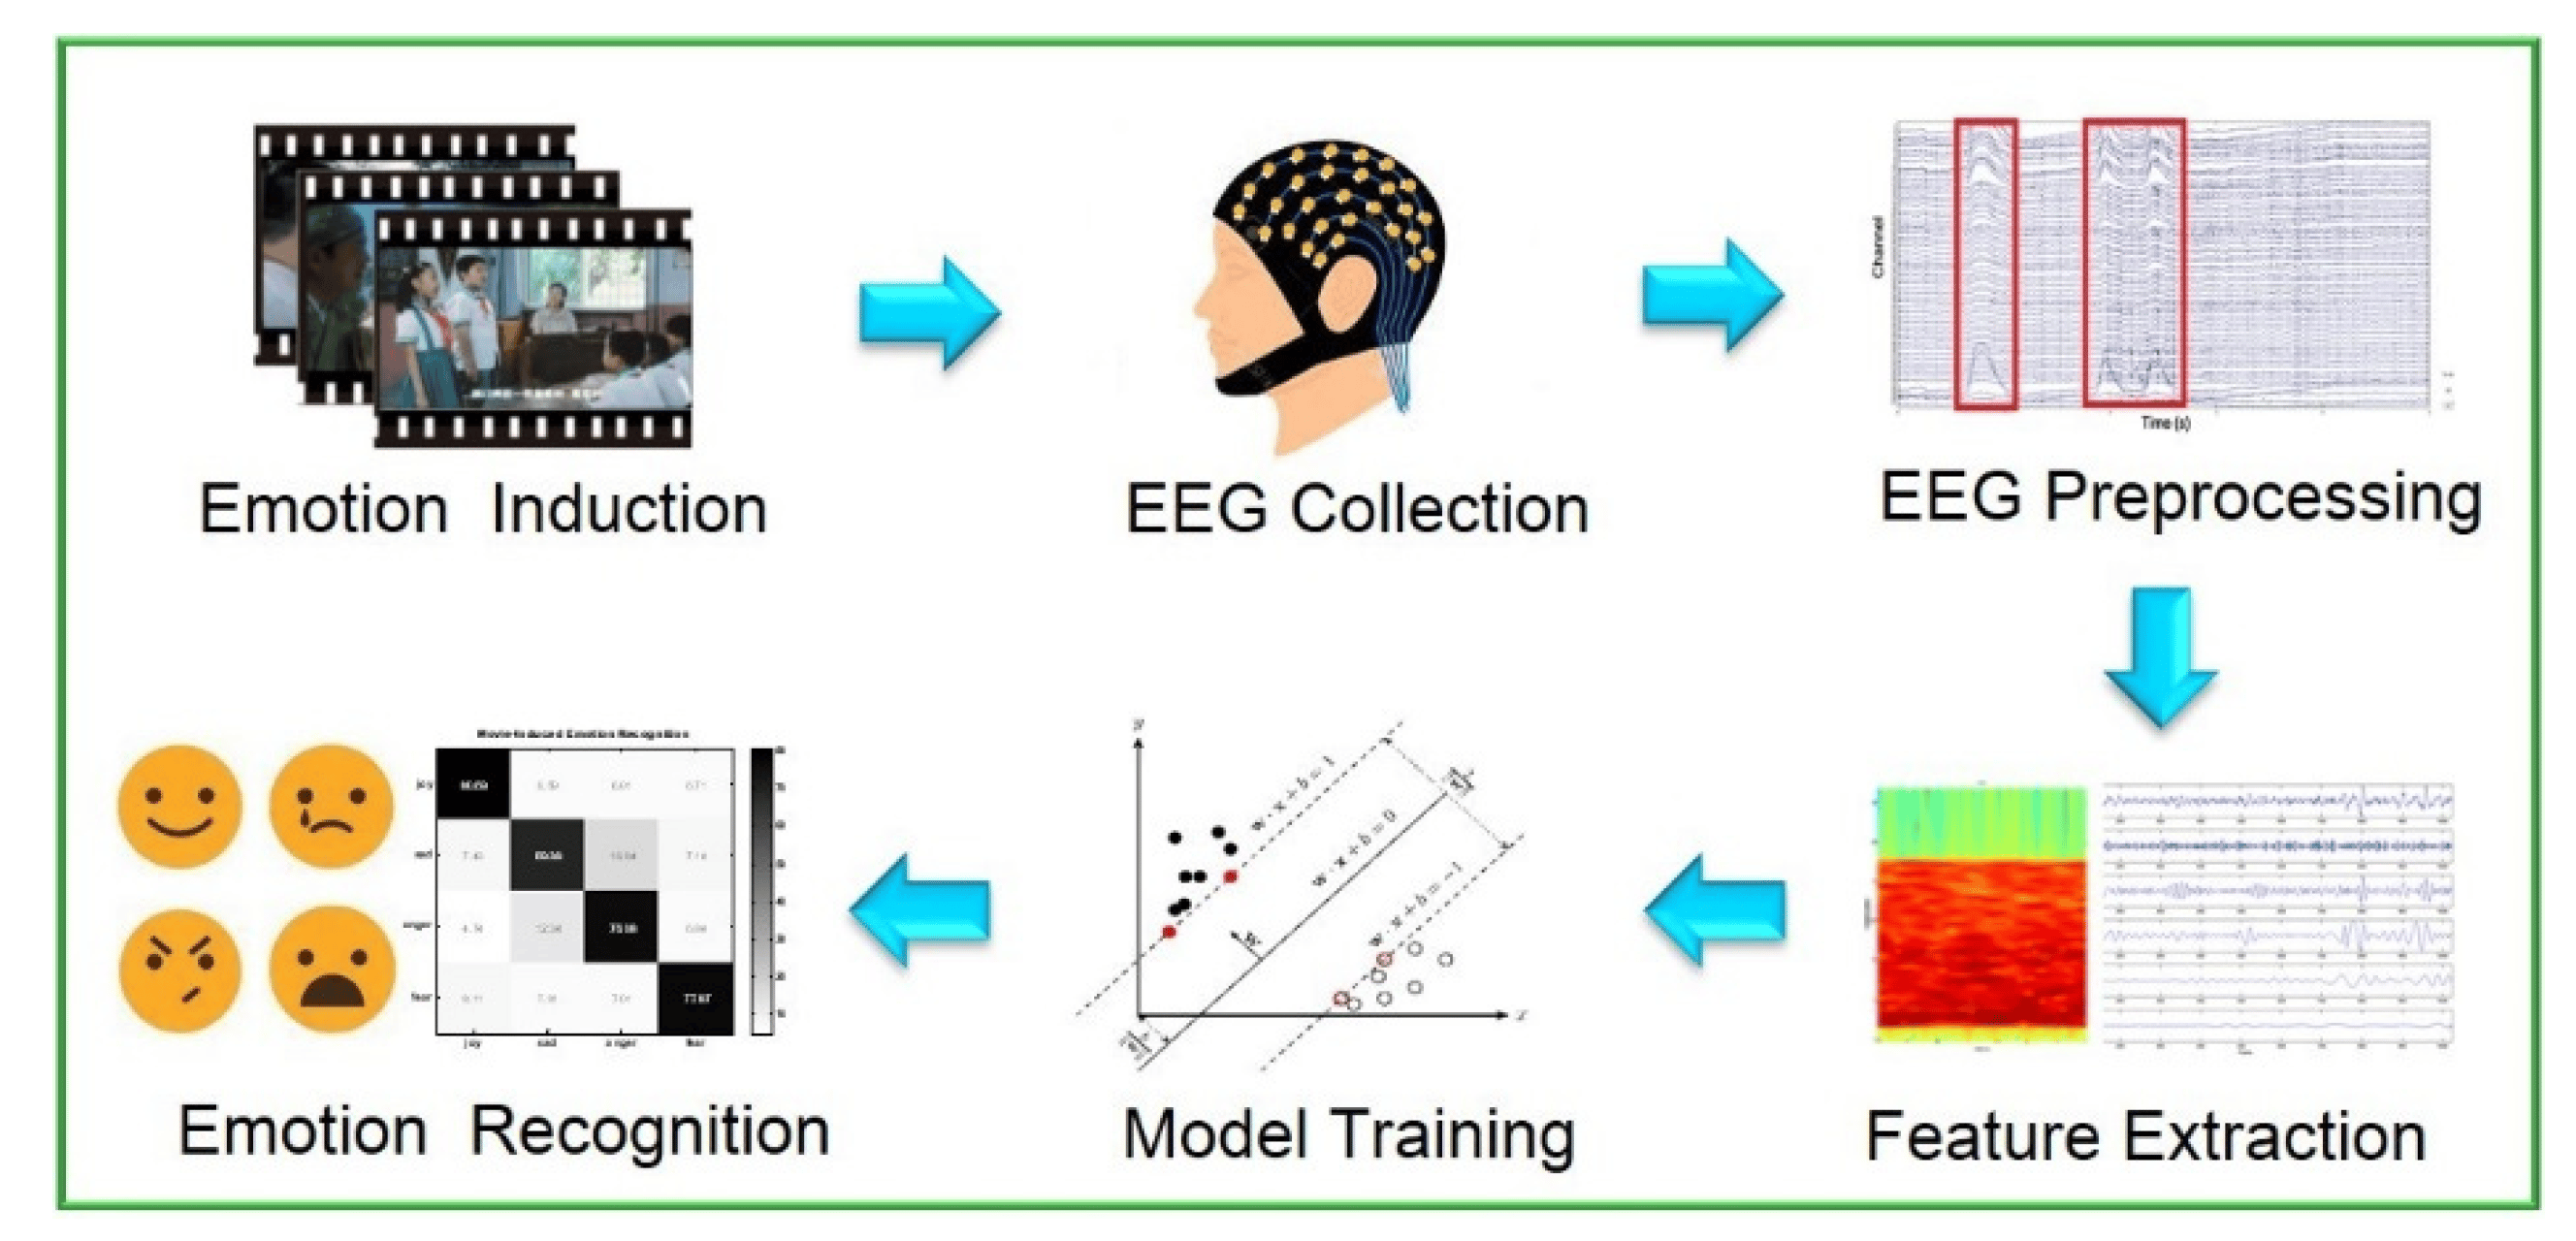
\includegraphics[scale=0.07]{EEG.png}} 
\caption{Emotion detection using EEG  \cite{zheng2023two}}
\label{fig}
\end{figure}
\cite{ma2022data}
EEG measures the electrical activity of the brain by placing electrodes on the scalp. EEG signals are recorded over time, resulting in a time-series data format. Participants are often exposed to stimuli that evoke different emotional responses, and their brain activity is recorded during these stimuli presentations. EEG signals are raw and complex time-series data. To make them suitable for machine learning algorithms, relevant features need to be extracted. Features can include spectral power, frequency bands (such as alpha, beta, theta), connectivity measures (like coherence or phase synchronization), and statistical features. These features capture different aspects of brain activity related to emotions. EEG data can be high-dimensional due to the large number of electrodes. Dimensionality reduction techniques like Principal Component Analysis (PCA) or feature selection methods are often applied to reduce the number of features and maintain only the most informative ones. Various machine learning and deep learning models can be used to predict emotions from EEG features. Some common models include Support Vector Machines (SVMs), Random Forests, Recurrent Neural Networks (RNNs), Convolutional Neural Networks (CNNs), and Long Short-Term Memory (LSTM) networks. The selected model is trained on labeled EEG data, where each sample is associated with an emotional label (such as happiness, sadness, anger, etc.). The model learns to map the extracted EEG features to the corresponding emotional states. The trained model is validated on a separate dataset that it hasn't seen during training. This helps assess the model's generalization ability and identify potential overfitting. Testing is then conducted on a completely unseen dataset to evaluate its performance in real-world scenarios. Once trained and validated, the EEG model can take new EEG data as input and predict the associated emotional state. The model's output could be a probability distribution over different emotions or a single predicted emotion label.

\section{Related Works}

The \cite{siriwardhana2020multimodal} shows the working of transformer self attention based architecture. \cite{makiuchi2021multimodal} shows the fusion of multimodal architecture, which ultimately provides higher accuracy with better results. \cite{ju2020transformer} positional encoding is added to the input embeddings to provide information about the word's position in the input sequence.
The accuracy of time-contextual learning's video emotion recognition can be increased with the use of an entirely novel network initialization technique.  A video multimodal emotion identification system based on an attention fusion network is suggested in order to get around the weight consistency of each modality in multi modal fusion \cite{huan2021video},\cite{abdullah2021multimodal}.

\begin{figure}[htbp]
\centerline{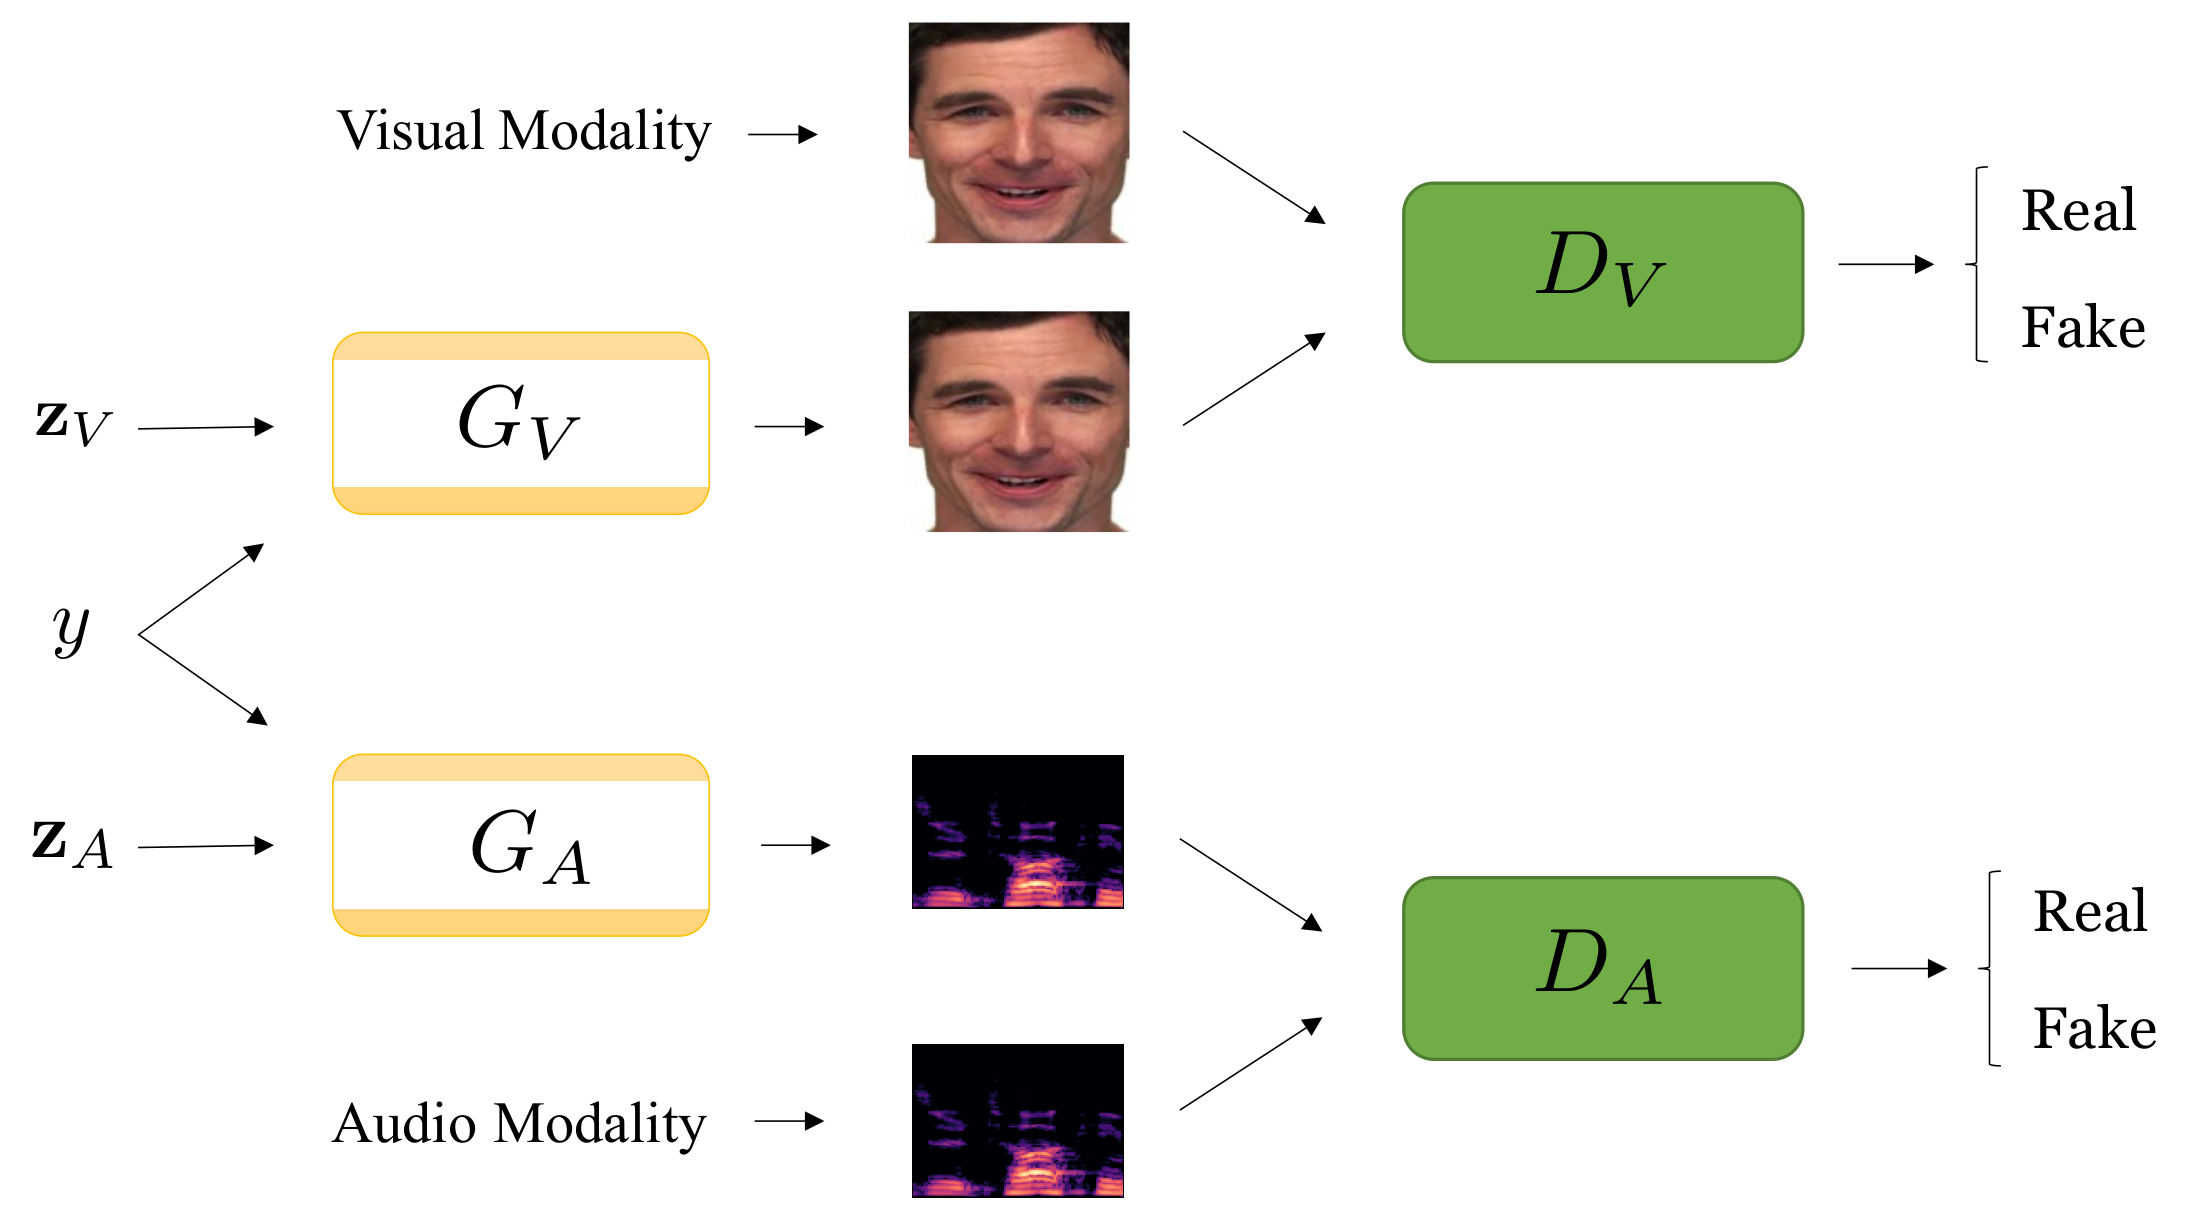
\includegraphics{GANs.png}}
\caption{Emotion detection using GANs \cite{KUMAR2022104483}}
\label{fig}
\end{figure}
\cite{ma2022data}

GAN stands for "Generative Adversarial Network," and it is a powerful framework in deep learning for generating new data that is similar to existing data. GANs consist of two neural networks, a generator and a discriminator, which are trained simultaneously through a competitive process. GANs can be used for image-to-image translation challenges when the emotion detection model benefits from having several visual representations of emotions. \cite{sharafi2022novel} GANs, can transform an image of a person's facial expression into different emotional expressions, resulting in a more diversified set of data for training the emotion recognition model. GANs can be used to produce visuals based on certain emotions. GANs can supplement training data for emotion detection models. GANs can assist increase the variety of the dataset by generating more synthetic samples, which can lead to better generalization and increased performance of the emotion detection model\cite{setyono2023data}. Sima et. al \cite{das2023emotion} had reviwed various advantages and disadvantages of GAN architecture for emotion detection.

\begin{figure}
\centerline{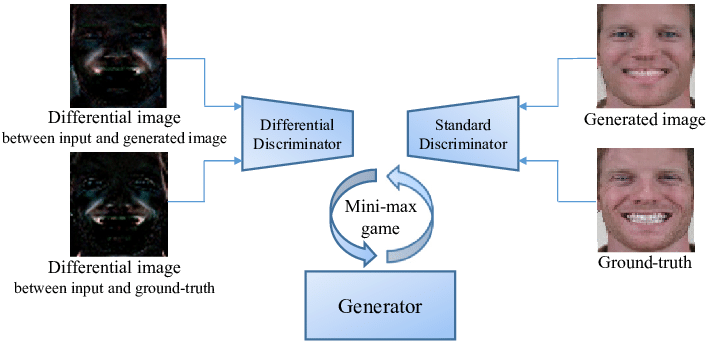
\includegraphics[scale=0.3]{GAN.png}}
\caption{GAN architecture for emotion detection \cite{article}}
\end{figure}

\cite{aldawsari2023optimizing} presented specialized EEG channel and feature selection techniques to exclude extraneous data from high-quality features. Haya et. al \cite{hasnul2023augmenting} presented The classification accuracy of five machine learning algorithms—the k-nearest neighbors (KNN), support vector machine, decision tree, random forest, and multilayer perceptron—is used to evaluate augmentation strategies. Mohan Karnati et. al \cite{karnati2023understanding} presented the survey for facial expression recognition (FER).

Gated Recurrent Unit (GRU) networks, like other recurrent neural networks (RNNs), can be used for emotion detection tasks, particularly when dealing with sequential data such as text or speech. GRUs are a form of RNN that overcomes some of the drawbacks of traditional RNNs, such as the vanishing gradient problem, which can make it difficult for the model to capture long-term dependencies in sequences \cite{maji2023multimodal}.


Bubai et. al \cite{electronics11091328} presented Mel-spectrograms  using the Conv-Cap module, and the remaining spectral characteristics from the input tensor were obtained using the Bi-GRU. Each module made use of the self-attention layer to identify the attention weight and preferentially concentrate on the best cues in order to produce high-level features. 
\begin{figure}
\centerline{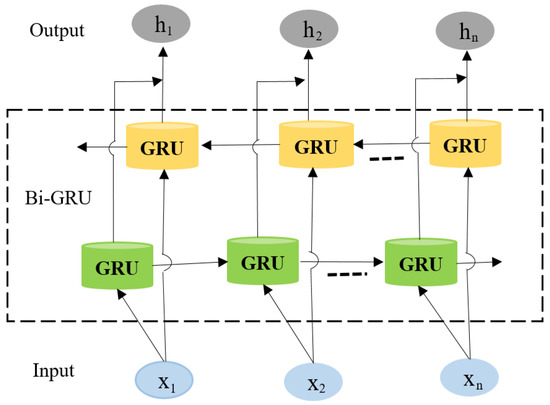
\includegraphics[scale=0.5]{GRU.png}}
\caption{GRU architecture for emotion detection \cite{electronics11091328}}
\end{figure}
 With the aid of six bidirectional gated recurrent units and two convolution layers (MBi-GRUMCONV), the model performs sentiment classification on vectorized reviews using two Word2Vec algorithms, namely the Skip Gram and Continuous Bag of Words, in three distinct vector sizes (100, 200, and 300) \cite{bacsarslan2023mbi}. \cite{han2023speech} A deep residual shrinkage network with bi-directional gated recurrent unit (DRSN-BiGRU) was proposed. A speaker emotion detection unit (SED-Unit), and a decoder with speaker emotion detection Bi-LSTM (SED-Bi-LSTM) was proposed \cite{liang2023mmateric}. In a bidirectional GRU, the input sequence is processed in both directions, forward and backward. This enables the model to capture information from both past and future contexts. Bidirectional GRUs are particularly useful for emotion detection tasks as they allow the model to understand the context surrounding each word in the sequence.

This research presents a novel emotion recognition system based on various modalities, such as electroencephalogram (EEG), galvanic skin response (GSR), and facial expressions \cite{cimtay2020cross},\cite{chowdary2022emotion}. In this concept, for each modality, a dedicated neural network is constructed to process the respective data \cite{liu2023multi}. The data is processed by modality-specific networks, and the features that were extracted are then integrated to produce a combined representation. \cite{priyadarshini2023emotion}, \cite{pan2023multimodal}
The hybrid LSTM/CNN model is used in this investigation. \cite{zhang2021multimodal},\cite{tzirakis2017end}. In order to improve the precision of feature extraction, the spatial and temporal features derived from video frames are fused together \cite{sharafi2022novel},\cite{gu2021multimodal}. Yun Gu et. al \cite{gu2023domain} presemted EEG model  for the intelligence and humanization of brain-computer interface (BCI). \cite{vempati2023systematic} presented a review on Brain-Computer Interaction (BCI) system intelligence has become more dependent on electroencephalogram (EEG)-based emotion recognition. 30 hearing-impaired participants who were watching video clips showcasing six different emotions—happiness, inspiration, neutral, anger, fear, and sadness—were asked to record their EEG activity in \cite{bai2023sect}

Hybrid neural network architecture was designed by U.M.Fernandes Dimlo et. al \cite{dimlo2023innovative}.

Transformers: \cite{nagarajan2023emotion} showed Emotion Recognition from Videos Using Transformer Models. \cite{le2023multi} presented transformer-based fusion and representation learning method to fuse and
enrich multimodal features from raw videos for the task of multi-label video emotion recognition. \cite{hsu2023applying} presented bi-modal transformer. \cite{wu2023transformer}  A large-scale self-collected physiological dataset was used to pre-train the SSL model, and three publicly available supervised emotion detection datasets were used to freeze or fine-tune the resultant encoder. \cite{kumar2023emotion} Word embedding is used to compare various machine learning and deep learning algorithms and show accuracy.

Transfer Learning: \cite{shehada2023lightweight} uggested to use a unique model that transfers features between datasets. With the help of this model, it is possible to apply characteristics discovered while resolving a limited number of challenging new situations. 


\section{Discussions}
The challenges in multimodal emotion detection include aligning data from different modalities.
Since emotions are very context-dependent, it is essential to accurately capture the context during emotion detection. Contextual data integration across several modalities is still an unsolved research issue.
Handling missing or noisy information, and designing effective fusion strategies to combine the modalities appropriately may be a challenging task to perform. \cite{liang2020semi}
Considerations for Multilingualism and Diversity Cultural and linguistic obstacles can affect how emotions are communicated and understood. Building models with universal applicability requires research into understanding and overcoming these differences.
While categorizing fundamental emotions (such as happiness and sorrow) is a common topic of current study, measuring the level of intensity or valence of emotions is still a difficult task.
Collecting accurate and reliable labeled data for training emotion detection models can be difficult. Emotions are often subtle and can be influenced by various contextual factors, making it challenging to determine the true emotional state of an individual.

Emotions can be expressed in various ways, and individuals may express the same emotion differently. Emotions are influenced by the context of the speech, and the same words spoken in different contexts can convey different emotions. Background noise and other acoustic disturbances can affect the accuracy of emotion detection. Collecting large and diverse emotion-labeled audio datasets can be challenging.

\cite{jia2022multimodal} GRU networks have the advantage of capturing long-term dependencies in sequential data. The GRU's update and reset gates enable it to manage the flow of information over time. The update gate aids valuable information from the previous time step, whereas the reset gate regulates how much historical information is forgotten. This gating mechanism allows GRU networks to learn patterns and dependencies across lengthy sequences.

\begin{center}
\begin{figure}
\centerline{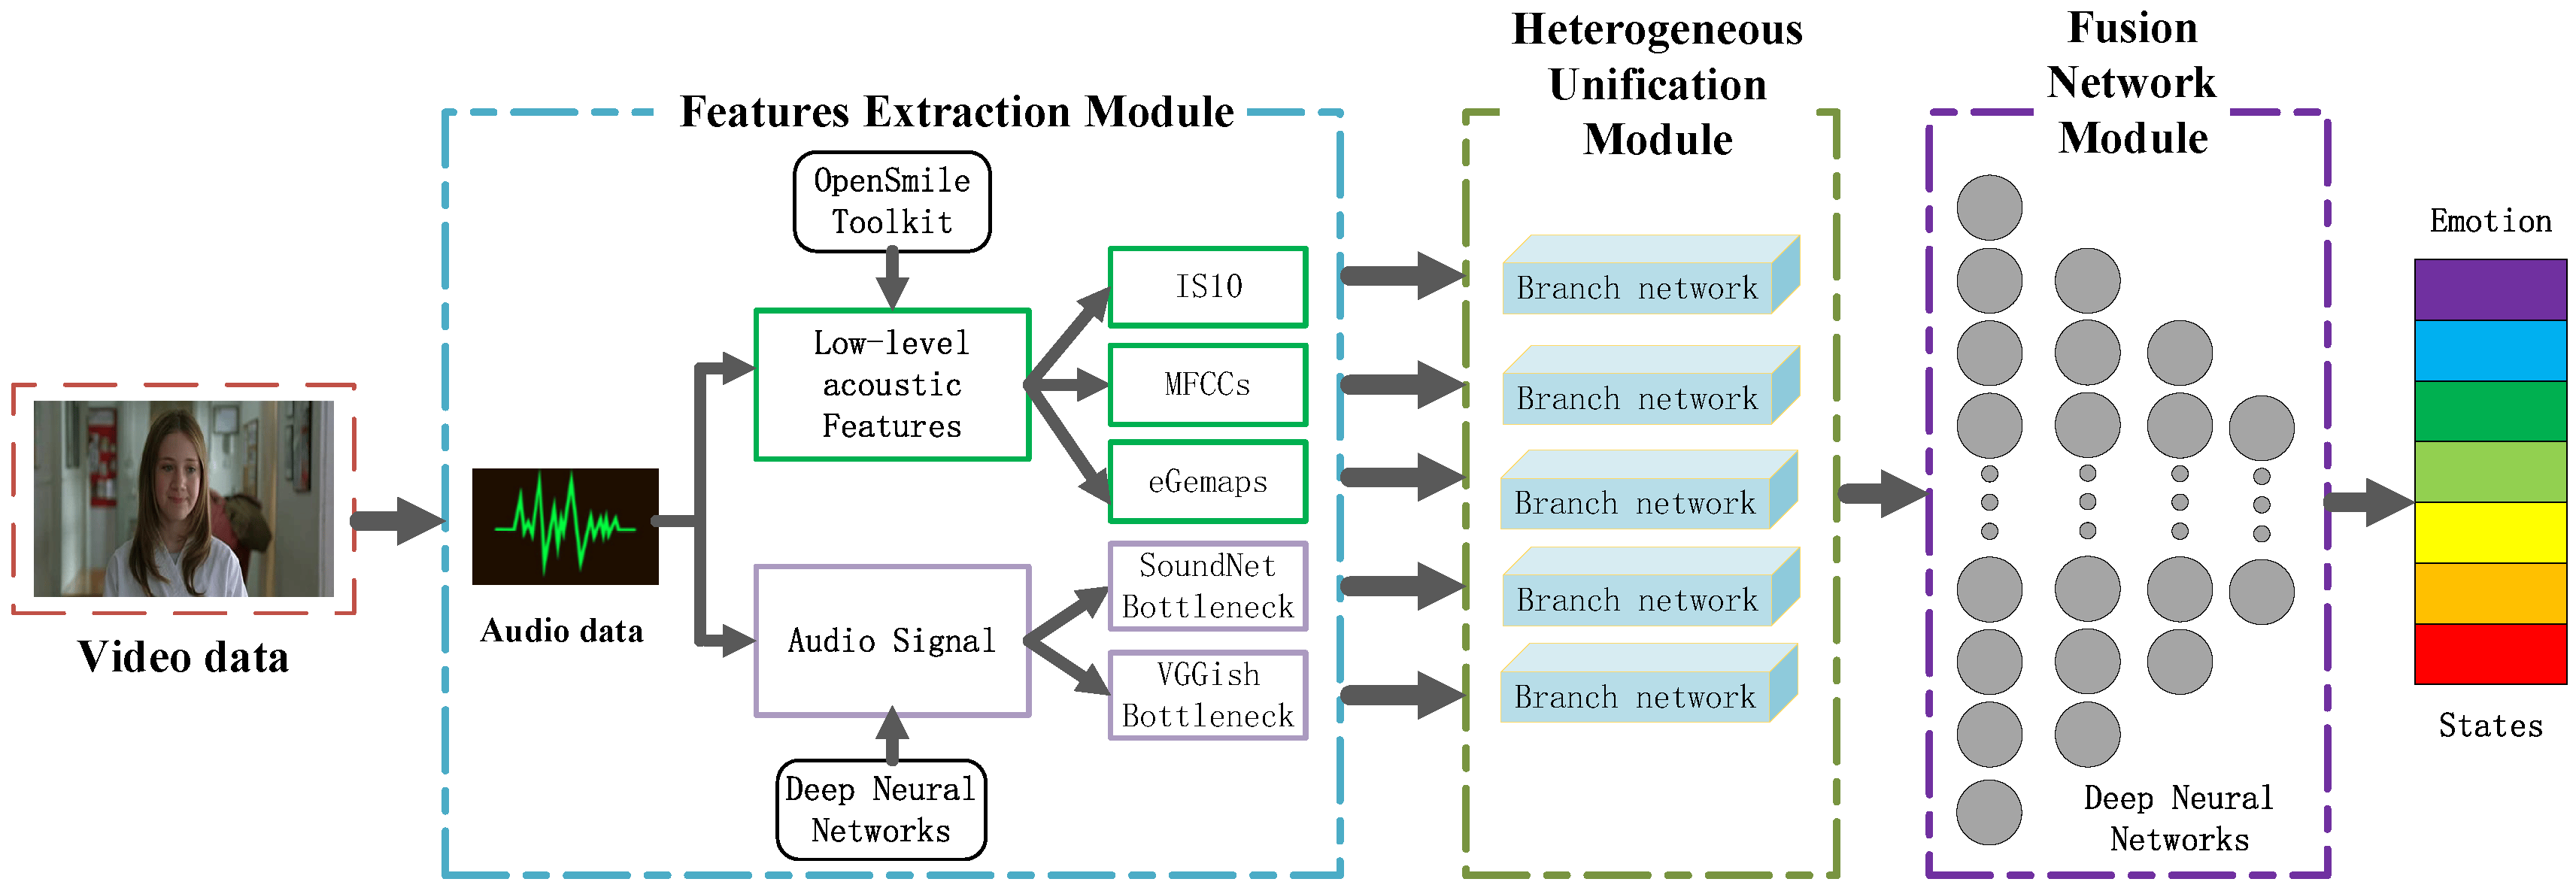
\includegraphics[width=0.5\textwidth]{DNN.png}}
\caption{Deep Neural Network architecture for Multimodal emotion detection \cite{s19122730}}
\end{figure}
\end{center}
Francesco Di Luzio et. al \cite{di2023randomized} had proposed the deep learning model  architecture employing parameter randomization in a complex classification model for emotion recognition. 

\newpage
\begin{center}
\section{Comparative Analysis}
\end{center}
\begin{longtable}
[h]
\begin{tabularx}{\textwidth}{|>{\raggedright\arraybackslash}X|>{\raggedright\arraybackslash}X|>{\raggedright\arraybackslash}X|>{\raggedright\arraybackslash}X|>{\raggedright\arraybackslash}X|}
\hline
References  & Findings  & Model  & Results & Critical Review \\

\hline
Multi modal Emotion Recognition based on Facial Expressions Speech, and EEG& 
GhostNet outperforms traditional classification models, demonstrating the clear superiority of proposed method. A tLSTM model that can better learn the emotional characteristics of each stage was designed The outcomes of our experiments on various publicly available datasets confirm the practicality of the proposed approach.& An LSTM model with a tree-like structure (referred to as tLSTM) that can integrate multi-stage features to extract emotional characteristics from EEG data. The improved GhostNet for facial expressions recognition.Architecture of tLSTM for EEG emotion recognition ,Architecture of LFCNN for speech emotion recognition & Paper introduces Deep-Emotion, a novel Multimodal Emotion Recognition (MER) method that leverages deep learning techniques for facial expressions, speech, and EEG. This approach includes an enhanced GhostNet for facial expressions, an LFCNN model for speech signals to reduce model size while maintaining accuracy, a tLSTM model for EEG signals, and an algorithm for optimal weight distribution for decision-level fusion.& At present, the research primarily relies on the examining  of publicly available datasets, and they haven't undertaken original data collection to validate the discoveries further.  There is a need to establish a standardized experimental framework for gathering data directly from participants, thereby Performing a more thorough assessment of the capabilities of Deep-Emotion.\\

\hline  
A systematic review on automated human emotion recognition using electroencephalogram signals and artificial intelligence &The provided content outlines a systematic review of automated emotion recognition from EEG signals using AI. It encompasses a range of topics, including EEG databases, preprocessing methods, feature extraction, and selection techniques. The review classifies studies into deep learning (DL) and machine learning (ML) categories for emotion identification systems. The analysis focuses on features, classification methods, classifiers, types of emotions classified, accuracy, and datasets used. While it presents a comprehensive overview of AI-based emotion recognition, specific findings or conclusions from the review are not available in this text. &The research paper employs deep learning models like CNN, DBN, RNN, and machine learning models including SVM, RF, DT, ANN, MLP, and kNN for EEG-based emotion recognition.&The conclusion summarizes the systematic review of emotion recognition from EEG signals using AI. It highlights the key findings, such as the preference for deep learning models, discusses the challenges in feature selection, and emphasizes the importance of understanding baseline EEG data. The review provides a valuable resource for researchers in the field of emotion classification, offering insights into databases, preprocessing methods, feature extraction, and classification methods. The work aims to guide the development of effective emotion classification systems utilizing Artificial Intelligence.&The more specific insights, especially about feature extraction and classifier selection, are needed. It highlights the potential for baseline EEG data and the importance of researching EEG-independent states. The review encourages further investigation into these aspects to enhance emotion recognition systems.  \\

\hline
Video multimodal emotion recognition based on Bi-GRU and attention fusion & The content presents a video multimodal emotion recognition method, emphasizing the effectiveness of combining Bidirectional Gated Recurrent Unit (Bi-GRU) and attention fusion to enhance accuracy. The approach overcomes weight consistency issues in multimodal fusion and improves recognition in single modalities. Key contributions include Bi-GRU-based time-contextual learning, novel network initialization, and real-time attention fusion for capturing multimodal contextual information. & The content discusses a multimodal emotion recognition model utilizing textual, visual, and audio data. It extracts and aligns features for recognition, but specific model details are not mentioned. &The research paper presents a time-contextual learning method utilizing Bi-GRU networks for improved video emotion recognition. It incorporates a new network initialization technique and a multimodal fusion approach based on the attention network to enhance accuracy. The study also suggests future work on high-dimensional audio features, stacked Bi-GRUs, hierarchical attention networks, and alternative fusion methods to further refine video multimodal emotion recognition&The provided content discusses a multimodal emotion recognition method based on Bi-GRU and attention fusion. The authors address issues of weight consistency in multimodal fusion and propose methods to enhance emotion recognition accuracy, particularly in the video context. The paper mentions significant contributions involving time-contextual learning, network initialization, and real-time attention mechanisms. It also claims superior performance compared to existing methods. \\

\hline
Transformer-based Label Set Generation for Multi-modal Multi-label Emotion Detection &The study confronts the complexity of detecting multiple emotions in multi-modal contexts within a single utterance. It underscores two significant factors: the impact of modality-to-label and label-to-label dependencies on emotion detection. To tackle these challenges, the researchers introduce a unified method called the multi-modal emotion set generation network (MESGN). MESGN integrates cross-modal interactions and temporal data through a transformer-based discriminative decoding process. It also leverages modality-to-label attention and self-critic learning techniques to enhance the performance of multi-label emotion detection& The emotion model consists of single-modal emotion set generation (SESGN) for each modality and a multi-modal emotion set generation network (MESGN) that captures cross-modal interactions and temporal information. The model uses transformer-based structures for encoding and decoding. &The results are provided in the form of performance metrics for different approaches to multi-modal multi-label emotion detection. MESGN outperforms various baseline approaches on both aligned and unaligned data, demonstrating the effectiveness of its approach in modeling multi-modal and multi-label dependencies. &The provided content does not include a critical review section. Typically, a critical review section would involve an analysis of the strengths and weaknesses of the proposed approach, a discussion of any limitations, and suggestions for further improvements. \\
\hline
Multi modal Emotion Recognition with Transformer-Based Self Supervised Feature Fusion &The study introduced a successful multimodal emotion recognition model utilizing Self-Supervised Learning (SSL) from various modalities, surpassing existing models on public datasets. It emphasized the importance of text features and revealed the significance of combining text and speech for sentiment analysis. Innovative fusion mechanisms (pre-IMA and post-IMA) enhanced the model's performance. Notably, the Hadamard product-based post-IMA fusion mechanism substantially improved sentiment accuracy. The study also identified a lack of prior research employing SSL features from diverse modalities in emotion recognition.  & The research innovatively employed "Transformer-based fusion" to integrate "Self-Supervised Learning (SSL) features" from diverse modalities, enhancing emotion recognition by amalgamating high-dimensional embeddings. & The section commences by elucidating the experiments carried out to assess the model's efficacy across the four datasets. The primary objective of this investigation is to devise a fusion mechanism capable of efficiently encapsulating input feature modalities through SSL features. The model's performance is juxtaposed with MuLT, an analogous multimodal fusion method, underscoring the advantageous attributes of SSL features. Additionally, it is noted that previous research endeavors have not emphasized the utilization of high-dimensional SSL features to encompass all modalities.& The study presented a holistic strategy for utilizing Self-Supervised Learning (SSL) features in multimodal emotion recognition. It excelled in designing fusion mechanisms and incorporating diverse SSL features from pre-trained models. Ablation studies provided insights into the importance of individual modalities and fusion components. This novel application of SSL techniques has practical implications for real-world contexts.\\
\hline
 Multimodal Emotion Recognition Using a Hierarchical Fusion Convolutional Neural Network&The paper introduces a novel Hierarchical Fusion CNN (HFCNN) model for multimodal emotion recognition, achieving high accuracy in classifying arousal and valence in both DEAP and MAHNOB-HCI datasets. Comparative results confirm HFCNN's superiority over other methods, although the paper lacks a detailed emotion model description and comprehensive discussion of limitations. &It discusses emotion recognition in terms of arousal and valence, which are common dimensions in emotion models. The HFCNN is applied to these dimensions to classify emotions&The results of the research paper indicate that the proposed Hierarchical Fusion CNN (HFCNN) model performs exceptionally well in multimodal emotion recognition. In the DEAP dataset, the model achieves an average accuracy of 83.28 PERCENT for arousal and 84.71 PERCENTfor valence, while in the MAHNOB-HCI dataset, it attains an accuracy of 88.28 PERCENT for arousal and 89.00 PERCENT for valence. These results outperform other state-of-the-art models when applied to the same datasets. The paper demonstrates the superiority of the HFCNN by highlighting its ability to extract hierarchical features and provide stable performance in recognizing emotions, particularly in the dimensions of valence and arousal. & The paper presents a novel approach for multimodal emotion recognition using the HFCNN model, which incorporates hierarchical fusion and deep learning techniques. The results are promising, with high accuracy in recognizing emotional states. However, the paper lacks a detailed description of the emotion model used and does not provide an extensive discussion of limitations and future work. It mentions the need for further research in areas such as cross-subject emotion classification, feature optimization, and neurogenic analysis, which indicates awareness of potential improvements. \\
\hline
Cross-Subject Multimodal Emotion Recognition Based on Hybrid Fusion & >The proposed hybrid multimodal emotion recognition method also increases the accuracy compared to using phys- iological modalities only. It increases the mean accuracy by approximately 13%. 
> Paper has achieved an average cross-subject high-low valence clas- sification accuracy of 86.6 PERCENT and an average high-low arousal classification accuracy of 84.7 PERCENT. & 2-D valence-arousal circumplex model &They introduce a subject-independent emotion recognition system designed for real-time operation, eliminating the need for feature extraction. This approach increases flexibility and reduces processing load. While EEG modality's subject-independent recognition accuracy is relatively low due to nonstationary properties, it is effective when dealing with a limited number of output classes. In this context, they restricted  the classes to two (high and low states for valence and arousal) to better capture the actual emotional state. & Future studies should prioritize subject-independent emotion recognition for broader, person-independent applicability. Emphasis should be placed on minimizing the number of modalities for practicality, and there should be a concerted effort to reduce the weight and form factor of sensor devices\\
\hline
End-to-End Multimodal Emotion Recognition Using Deep Neural Networks & >Due to memory and training instability concerns [45] it is not always optimal to use very large sequences in recurrent net- works. 
> model outperforms the other models in the test set when predicting the arousal dimension 
> The visual modality has been shown to more easily predict the valence dimension rather than the arousal. & Model using RECOLA database of the AVEC 2016 research challenge on emotion recognition. 
Output-Associative Relevance Vector Machine Staircase Regression 
And and the strength modeling system  
 & The models outperform others, including those submitted to the AVEC2016 challenge, when applied to the RECOLA database. They demonstrate the effectiveness of learning task-specific features. Furthermore, our multimodal model excels in both valence and arousal dimensions compared to other models. Future research could explore applying similar architectures for analysing behaviour in real-world scenarios. & Model can be expanded to include additional modalities, such as physiological data, to enhance its performance in emotion recognition tasks.  A wider range of emotion databases can be explored  including those with discrete emotion labels. \\
\hline
A Lightweight Facial Emotion Recognition System Using Partial Transfer Learning for Visually Impaired People &The proposed recognition model stands out as it achieves the highest recognition accuracy at 82.1 PERCENT on the FER2013 dataset, surpassing the current state-of-the-art. Notably, this model, with its 1.49 million parameters, is suitable for edge devices with constrained memory and processing capabilities. The model exhibits high accuracy in recognizing three labeled emotions—happy, sad, and surprise, while achieving a relatively lower accuracy for anger, disgust, and fear, with a notable rate of misclassification for the "sad" emotion. & A deep learning-based model for FER is proposed &The VIP dedicated system overcomes limitations of existing systems, offering a portable, lightweight, and accurate assistive solution. Evaluated on FER2013 and CK+, it achieved an 82.1 PERCENT accuracy on FER2013, a significant improvement over the current state-of-the-art, while maintaining computational efficiency. Additionally, it reached a 66.7 PERCENT accuracy on the CK+ test set, particularly excelling in recognizing happy, sad, and surprise emotions. & To improve recognition accuracy, it's advisable to train the model with more samples from the anger, disgust, and fear classes. Additionally, more work on deploying the FER system's prototype by integrating the trained FER model into a Raspberry Pi for further testing can be done\\
\hline
Multi-Label Multimodal Emotion Recognition With Transformer-Based Fusion and Emotion-Level Representation Learning &Proposed method outperforms baseline models and prior techniques, achieving an F1 score of 60.9 PERCENT and an accuracy of 85.9 PERCENT. Notably, their network supercedes all other approaches in terms of F1 score and exhibits a noteworthy accuracy improvement, surpassing the FE2E approach by +2 PERCENT. Moreover, this method significantly enhances performance on minority emotions such as anger, excitement, and happiness in the IEMOCAP dataset, and disgust, fear, and surprise in the CMU-MOSEI dataset. &> used a pre-trained ALBERT-base model to extract word embeddings from text transcription 
> video frames are sampled every 1s and then passed through a pre-trained MTCNN model to detect and crop the facial regions. &>This paper introduces a novel approach for multi-label multimodal emotion recognition, employing an end-to-end Transformer-based fusion technique for learning emotion-level representations. Unlike previous works that relied on hand-crafted features, proposed method takes raw video data as input. > They utilize multi-head attention within transformers to simultaneously combine the multimodal features of video data at different levels. Furthermore, they introduce a mechanism to learn emotion-level representations from the fused multimodal features, which enhances the model's performance in multi-label recognition tasks. & The visual modality (video frames) demands the most computational resources, which elongates the training process and impacts real-world applicability. Video sequences often contain redundant and nearly identical frames. There is work needed   for identifying and filtering out irrelevant and duplicated frames to lower the computational work thereby enhancing its practicality  \\
\hline
Continuous string data in cell 1 & Continuous string data in cell 2 & Continuous string data in cell 3 & Continuous string data in cell 4 & Continuous string data in cell 5 \\
\end{tabularx}
\end{longtable}
\newpage
\clearpage

\newpage
\section{Conclusion}

Multi modal emotion detection using machine learning is a fast expanding subject, and this overview study provides useful insights into the current state-of-the-art, obstacles, and future research possibilities. As multi modal data becomes more widely available, we anticipate that fusion of information from several modalities will continue to produce promising results, making substantial contributions to real-world applications. A detailed surrey of papers had been taken into consideration which gives the research possibilities in the field of Machine learning with applications on emotion detection. A critical analysis had been done how new techniques can be used to improve the results. 

\section*{Acknowledgments}
The author acknowledges the support and guidance of mentors and colleagues during the development of this research.

\bibliographystyle{unsrt}
\bibliography{BibTEXFILE}
\end{document}